\subsection{Broker}\label{sec:impl-broker}

The broker sub-system of our city simulator is written in Elixir, and leverages
Wabbit (a GenStage and RabbitMQ adapter).

\begin{figure}[H]
  \centering
  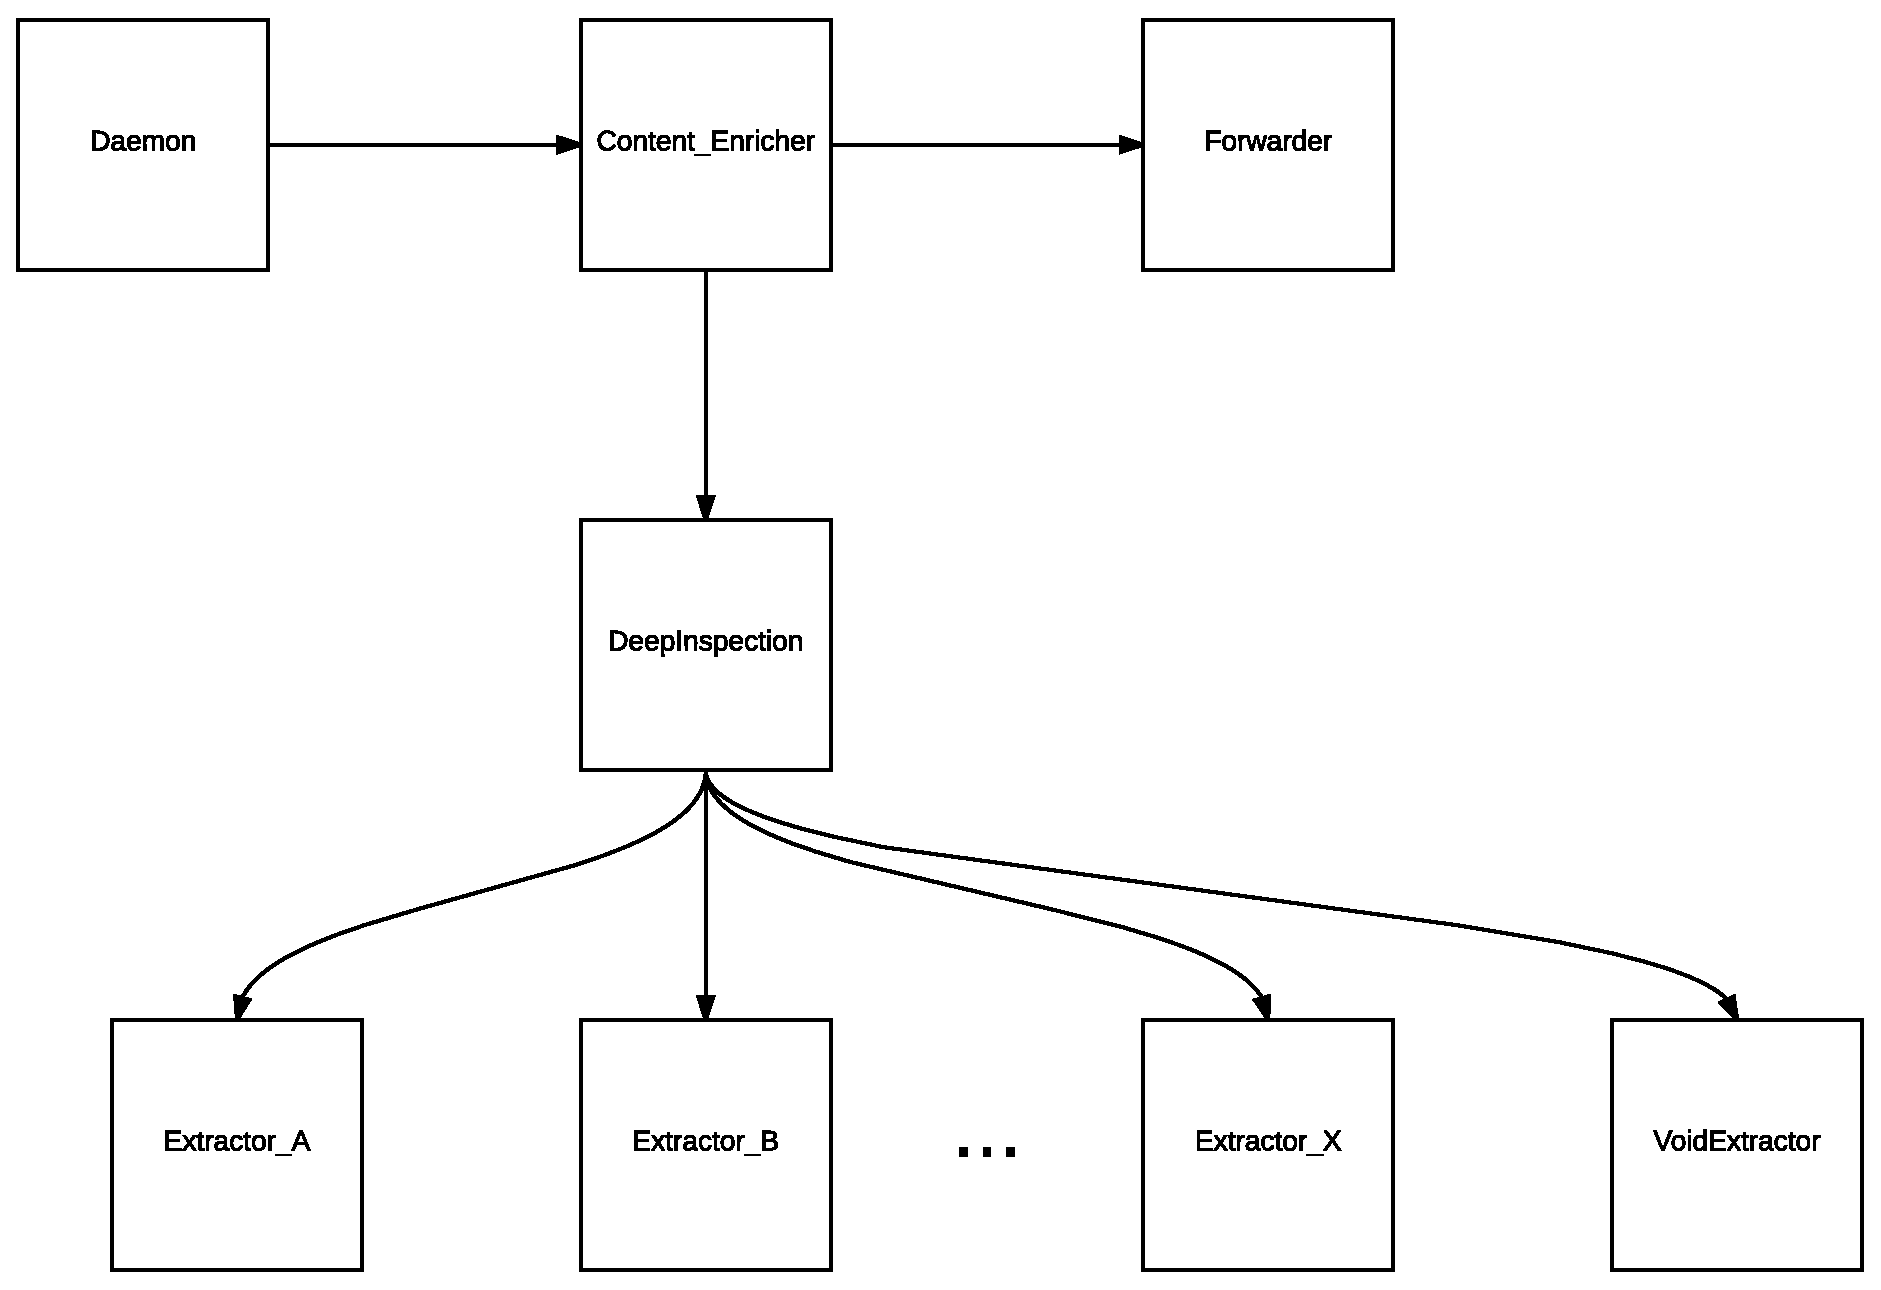
\includegraphics[width=\columnwidth]{images/implementation/broker.eps}
  \caption{Broker architecture}
  \label{fig:broker-arch}
\end{figure}

A broker is basically a pipeline through which messages are processed:

\begin{itemize}
  \item a \texttt{Daemon} process listens the RabbitMQ shared with the
    middleware nodes
  \item a \texttt{ContentEnricher} process 
  \item a \texttt{Forwarder} process puts messages on output queues of a
    RabbitMQ broker shared with the application server
\end{itemize}

Clearly, each one of this processes could be arbitrarily replicated, for
instance we may decide to have 3 \texttt{Daemon}s, 6 \texttt{ContentEnricher}s
and 8 \texttt{Forwarder}s, and this would be fairly trivial to implement.

On the other hand, one could also specialize these processes in order to
require to spawn an own replica to be able to cope with increased load. This
may be done by evaluating the processes' demand and offer variables, fixing
some thresholds and spawning other supervised workers on demand.

Each \texttt{ContentEnricher} transforms messages thanks to a
\texttt{DeepInspection} module, which indeed opens up the message and looks
inside to extract information.
It does so with the help of a series of Extractors modules\footnote{we did not
defined an Elixir Protocol, i.e., intereface for them but it would have been
quite easy} which actuate the process. There is also a \texttt{VoidExtractor}
module, which basically is a fallback case for an unidentified request.
